Mehr zu MVP (Model-View-Presenter) kann man \textit{\textbf{in folgende Quelle}} lesen.

Model-View-Presenter Architektur wird in den Anwendungen benutzt, die eine Oberfläche besitzen.
Die Architektur teilt die Anwendung in drei Teile:
\begin{itemize}
    \item \textbf{Model} - enthält die komplete Logik des Programms.
    \item \textbf{View} - empfängt alle Ereignisse von der Benutzeroberfläche (UI) und enthält die Daten, die angezeigt werden sollen.
    \item \textbf{Presenter} - transformiert die Daten in beide Richtungen vom Model zu View 
    und vom View zu Model
\end{itemize}


Eigenschaften der \textbf{MVP} Architektur:
\begin{itemize}
    \item \textbf{Presenter} und \textbf{Model} lassen sich mit Unittests abdecken.
    \item Jede neue \textbf{View} braucht einen eigenen \textbf{Presenter}.
\end{itemize}

\begin{figure}[H]
    \centering
    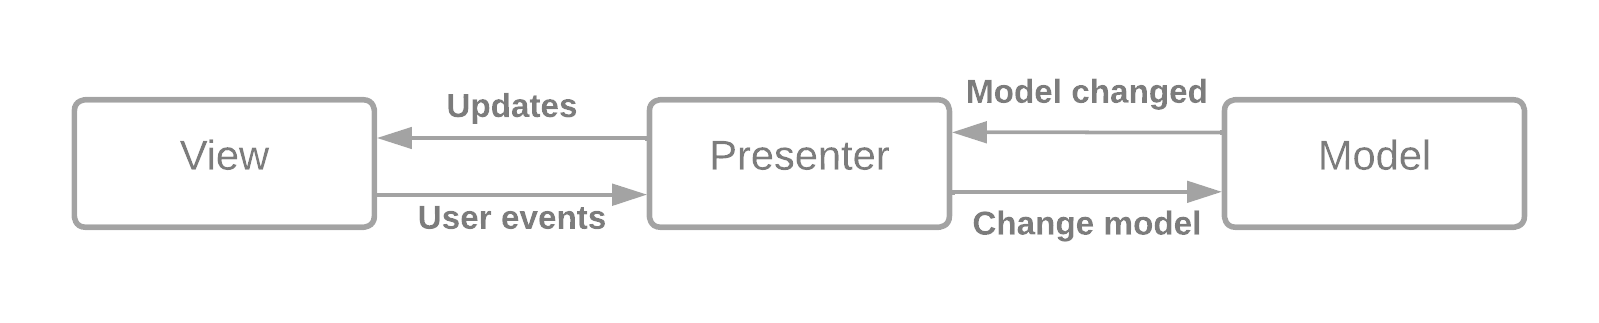
\includegraphics[width=1\textwidth]{./images/MVP.png}
    \caption[Datenfluss in MVP Architektur]{Datenfluss in MVP Architektur}
    \label{fig:MVP}
\end{figure}

Der Datenfluss in einer Anwendung, die mittels \textbf{MVP} implementiert ist, lässt sich wie folgt darstellen:
\begin{itemize}
    \item In der Oberfläche (\textbf{View}) wird ein Ereignis erzeugt(z.B. ein Button wurde gedrückt).
    \item \textbf{View} gibt das Ereignis an \textbf{Presenter} weiter.
    \item Das Ereignis wird im \textbf{Presenter} einem im \textbf{Model} definierten Ereignis zugeordnet(z.B. Button ``Speichern'' wurde gedrückt)
    \item Das \textbf{Model} bearbeitet das Ereignis (z.B. die Datei wurde gespeichert) und gibt das Ergebnis zurück.
    \item \textbf{Presenter} empfängt das Ergebnis (z.B. die Datei wurde erfolgreich gespeichert) und wandelt das in ein Ereignis,
    das \textbf{View} interpetieren kann (z.B. Button ``Speichern'' soll grün werden).
    \item \textbf{View} abarbeit das Ergebnis und zeigt es an (z.B. Button wird grün auf der Oberfläche angezeigt)
\end{itemize}